\section{Convolutional Neural Network}
上节课中,我们提到了深度学习的三种网络结构:线性分类器,多层感知机和卷积神经网络.下面我们首先介绍卷积层.

假定输入是$W_1 \times H_1 \times C$的矩阵,可以看作一张图片的宽度,高度,通道数.卷积层需要四个超参数:filter的数量$K$和大小$F$,步长$S$和零填充参数$P$.经过卷积层后,原本的输入变成$W_2 \times H_2 \times K$,其中
\begin{equation}
	\begin{split}
		W_2 = \frac{W_1 - F + 2P}{S} + 1
		\\
		H_2 = \frac{H_1 - F + 2P}{S} + 1
	\end{split}
\end{equation}
一共需要$F^2CK+K$个参数,其中额外的$K$是每层的bias.
\begin{comment}
	\begin{boxdef}{kernel和filter的区别是什么?}
		filter更多指filter layer,而kernel指卷积核这一weight matrix
	\end{boxdef}
\end{comment}


选用卷积核,可以降低feature map的大小.如果直接将图片进行flatten,将会导致大量信息的丢失.

所谓池化操作,就是一种降采样,可以降低图片的大小.比如采用$2\times 2$的大小进行最大值池化,就是将每个$2\times 2$范围内最大的像素的值作为池化后这个像素的取值,将原来的图片缩减到四分之一大小.池化可以增大感受野.虽然可以通过步长大于一的卷积来代替池化,但是池化不需要参数,更容易优化.

假定输入是$W_1 \times H_1 \times C$的矩阵,则池化层需要两个超参数:大小$F$和步长$S$.池化结果是产生$W_2 \times H_2 \times K$的矩阵,其中
\begin{equation}
	\begin{split}
		W_2 = \frac{W_1 - F}{S} + 1
		\\
		H_2 = \frac{H_1 - F}{S} + 1
	\end{split}
\end{equation}
池化层无需参数.

\begin{comment}
	\begin{figure}[htbp]
		\centering
		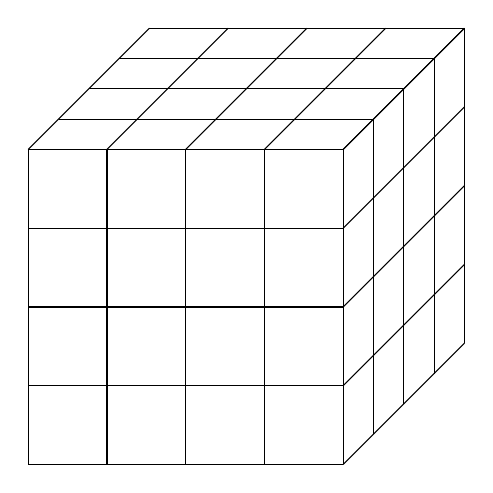
\begin{tikzpicture}
			\foreach \x in{0,...,4}
			{   \draw (0,\x ,4) -- (4,\x ,4);
				\draw (\x ,0,4) -- (\x ,4,4);
				\draw (4,\x ,4) -- (4,\x ,0);
				\draw (\x ,4,4) -- (\x ,4,0);
				\draw (4,0,\x ) -- (4,4,\x );
				\draw (0,4,\x ) -- (4,4,\x );
			}
		\end{tikzpicture}
		\caption{Caption}
		\label{fig:my_label}
	\end{figure}
\end{comment}
基于CNN的分类网络总结:ConvNets堆叠了卷积层,池化层和全连接层,倾向于使用更小的卷积核和更深的网络结构,尽量避免使用池化层和全连接层(只使用Conv层).其网络结构大致如下:
$$\texttt{[(Conv-ReLu)*N-Pool?]*M-(FC-ReLu)*K-SoftMax}$$
其中$N$一般不超过5,$M$比较大,$0\le K \le 2$.但最近的网络如ResNet,GoogleNet等也开始突破这些范围.

MLP与CNN的比较

如果输入为$W_1 \times H_1 \times C$的矩阵,输出$W_2 \times H_2 \times K$的矩阵,那么FC需要$W_1W_2H_1H_2CK$个参数,一层卷积核大小为$F$的CNN需要$F^2CK$个参数.后者一般比前者小得多.

对于一维情形,$h \in \mathbb R^m, x\in \mathbb R^n$,则$y = h * x$可以被表示为矩阵乘法:

\begin{equation}
	y=h * x=
	\begin{pmatrix}
		h_{1} & 0 & \cdots & 0 & 0 \\
		h_{2} & h_{1} & & \vdots & \vdots \\
		h_{3} & h_{2} & \cdots & 0 & 0 \\
		\vdots & h_{3} & \cdots & h_{1} & 0 \\
		h_{m-1} & \vdots & \ddots & h_{2} & h_{1} \\
		h_{m} & h_{m-1} & & \vdots & h_{2} \\
		0 & h_{m} & \ddots & h_{m-2} & \vdots \\
		0 & 0 & \cdots & h_{m-1} & h_{m-2} \\
		\vdots & \vdots & & h_{m} & h_{m-1}\\
		\vdots &\vdots & \cdots  &0 & h_{m}
	\end{pmatrix}
	\begin{pmatrix}
		x_{1} \\
		x_{2} \\
		x_{3} \\
		\vdots \\
		x_{n}
	\end{pmatrix}
\end{equation}

左侧的矩阵被称为Toeplitz矩阵.由于深度学习当中的卷积参数是学习而来,故不需要像传统的卷积操作一样进行翻转.二维情形的卷积则是一个double block circulant matrix.

由于我们选取较小的卷积核,所以前后层网络之间的连接更为稀疏.而且有更加明显的Parameter Sharing效应,即对每块区域采取相同的参数进行处理.

那么,FC和CNN两者哪个表达能力更强呢?很显然是FC更强,因为FC的表达范围是CNN的超集.但事实上,使用Conv的结果远好于FC/MLP.那么问题出在哪里呢?

一个显而易见的答案是,FC需要的参数量过于庞大了,一层可能需要上亿甚至更多的参数,这使得其非常难以被优化.另外一个非常重要的原因是,它并没有突出我们在视觉任务中目标的特点,即等变性(equivariance).

我们知道,在目标分类等任务当中,将图片进行轻微平移,旋转,改变亮度等操作,并不会影响结果.但是,它们都改变了输入的几乎每一个值.而即使移动了一个像素,FC的输出都将天差地别.换言之,我们要求FC将在它看来输出完全不同的的图像归为一类,这样的矩阵是非常难以寻找的,会在优化过程中产生极大的困难.

那么CNN的表现如何呢?我们先解释上文equivariance的含义.其一般定义为:
\begin{equation}
	S_A[\phi(X)] = \phi[T_A(X)]
\end{equation}
这里$A$指代某种操作,而$T_A, S_A$分别代表$X,\phi(X)$空间下的变换.例如将$A$看作左移一像素,忽略边界就有$T[\phi(X)] = \phi[T(X)]$.不变性是等变性在$S_A = I$的特殊情形.

我们需要指出的是,在这里Parameter Sharing就等同于Equivariance to Translation.我们用同样的参数处理每一个局部,那么忽略掉边界后,2D Conv就是等变的.

举个例子,当处理图像的时候,在第一个卷积层进行边的探测是非常有用的,而同样的边或多或少地会出现在图片的其他位置,所以在整个图片范围内进行参数共享是非常可行的操作.换言之,对于反映同种信息的pixel的识别,在不同位置应该是相同的,这种人类视觉给出的先验知识才是Conv的根本思路.

但需要强调的是,Conv并不是万能的,一个layer作为一个函数,其需要具有何种性质与目标的性质高度相关.我们使用CNN正是因为当前我们的目标具有这种不变性.但有时你需要位置相关的处理,比如统计一张照片上的绵羊数量,那显然就不能将不同地方的绵羊做相同处理.这方面的工作就是semi-Conv的工作,发表于CVPR 2018.同样,它也不具有图像缩放,图像旋转等情形下的不变性,需要引入其他机制进行处理.